\documentclass{article}

% if you need to pass options to nat, use, e.g.:
%     \PassOptionsToPackage{numbers, compress}{natbib}
% before loading neurips_2018

% ready for submission
% \usepackage{neurips_2018}

% to compile a preprint version, e.g., for submission to arXiv, add add the
% [preprint] option:
%     \usepackage[preprint]{neurips_2018}

% to compile a camera-ready version, add the [final] option, e.g.:
\usepackage[final,nonatbib]{nips_2018}

% to avoid loading the natbib package, add option nonatbib:
% \usepackage[nonatbib]{nips_2018}

\usepackage[utf8]{inputenc} % allow utf-8 input
\usepackage[T1]{fontenc}    % use 8-bit T1 fonts
\usepackage{hyperref}       % hyperlinks
\usepackage{url}            % simple URL typesetting
\usepackage{booktabs}       % professional-quality tables
\usepackage{amsfonts}       % blackboard math symbols
\usepackage{nicefrac}       % compact symbols for 1/2, etc.
\usepackage{microtype}      % microtypography
\usepackage[square,numbers]{natbib}
\usepackage{graphicx}
\usepackage{subcaption}

\title{Detecting Breast Cancer with Supervised Learning Techniques}

% The \author macro works with any number of authors. There are two commands
% used to separate the names and addresses of multiple authors: \And and \AND.
%
% Using \And between authors leaves it to LaTeX to determine where to break the
% lines. Using \AND forces a line break at that point. So, if LaTeX puts 3 of 4
% authors names on the first line, and the last on the second line, try using
% \AND instead of \And before the third author name.

\author{%
  Matt Dietrich \\
  50981794 \\
  University of British Columbia \\
  \texttt{dietrich@alumni.ubc.ca} \\
  \And
  Arun Rajendran \\
  86611860 \\
  University of British Columbia \\
  \texttt{arun95@math.ubc.ca} \\
  % \AND
  % Coauthor \\
  % Affiliation \\
  % Address \\
  % \texttt{email} \\
  % \And
  % Coauthor \\
  % Affiliation \\
  % Address \\
  % \texttt{email} \\
  % \And
  % Coauthor \\
  % Affiliation \\
  % Address \\
  % \texttt{email} \\
}

\begin{document}
% \nipsfinalcopy is no longer used

\maketitle

\begin{abstract}
  Because many different machine learning approaches can be applied to the field of healthcare, it is important to identify which techniques perform well on a specific task. We target the task of breast tissue tumour classification and compare the performance of several supervised learning classifiers on cancer detection. As a supplementary approach, we also explore unsupervised dimension reduction techniques to visualize the dataset and search for distinguishable clustering. Although each tested classifier performs well, we observe that random forest classifiers yield the lowest test error on average and therefore seem to be best suited to the tumour classification problem.
\end{abstract}

\section{Introduction}

% Context

Healthcare is a critical pillar of society that continues to drive and leverage advancements in technology. As the availability of data improves, machine learning is increasingly applied to many challenges in the field. The use of machine learning is justified for several reasons, such as the potential for faster medical diagnoses with reduced human error.

% Importance of the problem

Given the plethora of machine learning algorithms available, it is important to understand which techniques are best suited to a specific healthcare related task (such as the diagnosis of cancer). Because early detection provides more time for the delivery of potentially life-saving treatment, it is especially critical to identify and apply high performing classification methods.

% Summarize Contribution

In this project, we focus on the classification of tumours as malignant (cancerous) or benign (noncancerous). We evaluate the performance of several supervised learning techniques in classifying breast tissue tumours in the Wisconsin breast cancer diagnostic dataset retrieved from the UCI Machine Learning repository \cite{uci2017}. The classifiers we consider are random forests, k-nearest neighbours, naive Bayes, support vector machines, and neural networks. 

Our primary contribution is the following: we observe that each of the tested classifiers performs fairly well after hyperparameter tuning, with errors below 10\%. The random forest classifier yields the lowest test error on the dataset and therefore seems to be the best suited classifier for this task.

As a complement to the classifier comparison, we also explore unsupervised dimensionality reduction similar to Jamieson et al. \cite{tsne2010}. We plot the two-dimensional results of principal component analysis, multi-dimensional scaling, ISOMAP, and t-distributed stochastic neighbour embedding. Our visualizations show distinguishable clustering of the data, with several mixed regions. We conclude therefore that unsupervised dimensionality reduction techniques could potentially lend support to a supervised learning classification decision but are unlikely to be sufficient on their own. 

\section{Related Work}

Polat and Guines \cite{POLAT2007694} conducted breast cancer diagnosis using least square support vector machine (LS-SVM) classifier algorithm and showed that it achieves close to 98\% accuracy. Jose et al. \cite{JEREZ2010105} evaluated the performance of several statistical and machine learning imputation methods that were used to predict recurrence in patients in an extensive real breast cancer data set.
Kourou et al. \cite{KOUROU20158} presented a review of recent machine learning approaches employed in the modeling of cancer progression. Akay \cite{AKAY20093240} proposed breast cancer diagnosis based on a SVM-based method combined with feature selection and showed that it has highest classification accuracy (99.51\%) when the model contains five features. 

Wolberg et al. \cite{WOLBERG1994163} develoed an interactive computer system that evaluated and diagnosed breast cancer based on cytologic features derived directly from a digital scan of fine-needle aspirate (FNA) slides. They trained their system on data provided by 569 patients and used samples given by additional 54 consecutive, new patients to test the system. They have shown that the projected prospective accuracy of the system estimated by tenfold cross validation was 97\% and the actual accuracy on test dataset consisting of 54 new samples (36 benign, 1 atypia, and 17 malignant) was 100\%. They also stated that the digital image analysis coupled with machine learning techniques will improve diagnostic accuracy of breast fine needle aspirates.

These works indicate that high levels of accuracy can be achieved using machine learning algorithms. Most of the works have focused on one particular algorithm and have presented their validation and test results for this algorithm. In our project, we present a comparative study of different supervised machine learning techniques and identify the best algorithm that is suitable for the breast cancer dataset. We believe that this step has to be done before hyperparameter tuning and cross-validation to achieve optimal accuracy gains.

\section{Methods}

\subsection{The Dataset}

Our analysis focuses on the Wisconsin breast cancer diagnostic dataset retrieved from the UCI Machine Learning repository \cite{uci2017}, originally used in previous work \cite{tumour:1993}. The features in the dataset are calculated from microscope images of breast tissue masses. The following features are included for each of the 569 examples:

\begin{itemize}
\item ID number
\item Diagnosis, where M = malignant (cancerous) and B = benign (noncancerous)
\item Ten numerical features are computed for each cell nucleus, described in further detail in the original paper \cite{tumour:1993}:

\begin{itemize}
	\item Radius (defined as the mean of distances from center to points on the perimeter)
	\item Texture (defined as the standard deviation of gray-scale values)
	\item Perimeter (defined as the distance around the shape)
	\item Area (defined as the size of the shape interior)
	\item Smoothness (defined as the variation in radius lengths)
	\item Compactness (defined as the perimeter squared divided by the area)
	\item Concavity (defined as the magnitude of concave portions of the contour)
	\item Concave points (defined as the number of concave portions of the contour)
	\item Symmetry (defined as the length difference between lines perpendicular to the longest chord in the cell)
	\item Fractal dimension (defined as the rate of change of measured perimeter as the ruler size increases)
\end{itemize}

\end{itemize}

For each of the above ten features, the dataset includes a mean, standard error, and a maximum value for each example. This provides a total of 30 features.

In our experiments, we discard the ID number as an irrelevant feature and use the diagnosis as our class label. We map malignant (cancerous) to 1 and benign (noncancerous) to 0.

We believe machine learning techniques can help with this dataset because it includes numerical features used by medical practitioners to diagnose tumours and was proven to yield a high performing decision tree classifier in previous work \cite{tumour:1993}.

\subsection{Supervised Learning Classifiers}

We conduct our main performance evaluation on a variety of common machine learning techniques. Specifically, we apply random forests, k-nearest neighbours, naive Bayes, linear support vector machines, and neural networks to the dataset. We survey a broad selection of supervised learning classifiers because of our goal to discover the best performing techniques for the tissue diagnosis problem.

\subsection{Unsupervised Dimension Reduction Techniques}

Secondarily, we use unsupervised dimension reduction techniques to provide complementary analysis. We apply principal component analysis, multi-dimensional scaling, ISOMAP, as well as t-distributed stochastic neighbour embedding to the entire dataset. Our intention here is to visualize the dataset in two dimensions to look for any observable clustering. Again, we choose to apply several techniques in a broad survey to search for the most useful visualization for this specific application.

\section{Experiments and Evaluation}

\subsection{Supervised Learning Classifier Comparison}

Our primary experiment consists of the performance evaluation of several supervised learning techniques on the breast cancer dataset.

We begin by randomizing the order of the 569 examples and split the dataset so that we have 80\% of the examples for training and 20\% of the examples set aside for testing. Next, we tune a selection of hyperparameters for each model using grid search with 5-fold cross-validation. Hyperparameters tuned are summarized in Table \ref{tab:hp}.

\begin{table}[]
	\caption{Hyperparameters tuned for each supervised learning classifier}
	\label{tab:hp}
	\centering
	\begin{tabular}{ll}
		\toprule
		Classifier  			& Hyperparameters Tuned \\
		\midrule
		Random forests 	& number of estimators \\
		k-nearest neighbours   & number of neighbours \\
		Gaussian naive Bayes & variance smoothing \\
		Linear support vector machines & C (error term penalty)\\
		Neural networks & hidden layer sizes \footnotemark \\
		& alpha (L2 regularization parameter) \\
		\bottomrule
		
	\end{tabular}
\end{table}
\footnotetext{We consider only one hidden layer in our neural network analysis.} 

We repeat the experiment (including randomizing the dataset order) 10 times and take the mean test error for each classifier to limit irregularities arising from the random test set selection. Our intention is to identify the method or methods that perform the best for this particular application. Average classification error for each classifier is summarized in Figure \ref{fig:error}.

\subsection{Unsupervised Dimension Reduction Visualization}

Our secondary analsysis consists of unsupervised dimesion reduction of the dataset. We proceed to directly transform the full 569 examples in dataset into two dimensions. Our intention is to look for any observable clustering in the dataset that could support classification. Results of these two-dimensional visualizations are shown in Figure \ref{fig:viz}.

\begin{figure}
	\centering
	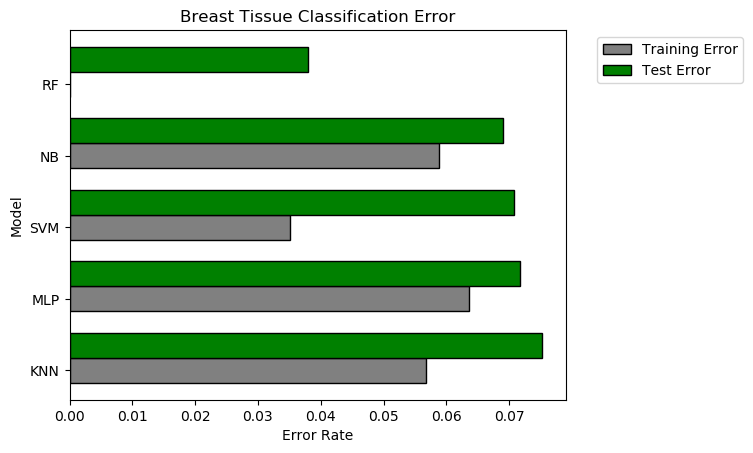
\includegraphics[width=1\textwidth]{../figs/classification_error_1_10_trials}
	\caption{Average classification error after hyperparameter tuning. Model name abbreviations are the following: RF = random forest; NB = Gaussian naive Bayes; SVM = linear support vector machine; MLP = multilayer perceptron (neural network); KNN = k-nearest neighbours.}
	\label{fig:error}
\end{figure}

\begin{figure}
	\centering
	\subcaptionbox{Principal component analysis}{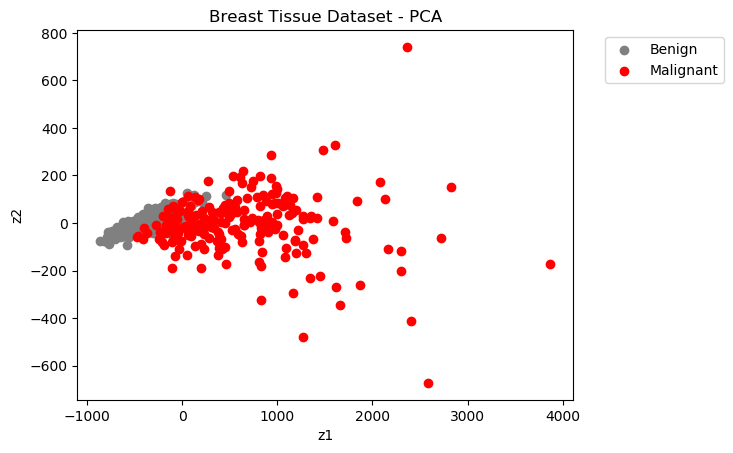
\includegraphics[width=0.49\textwidth]{../figs/pca_1}}
	\subcaptionbox{Multi-dimensional scaling}{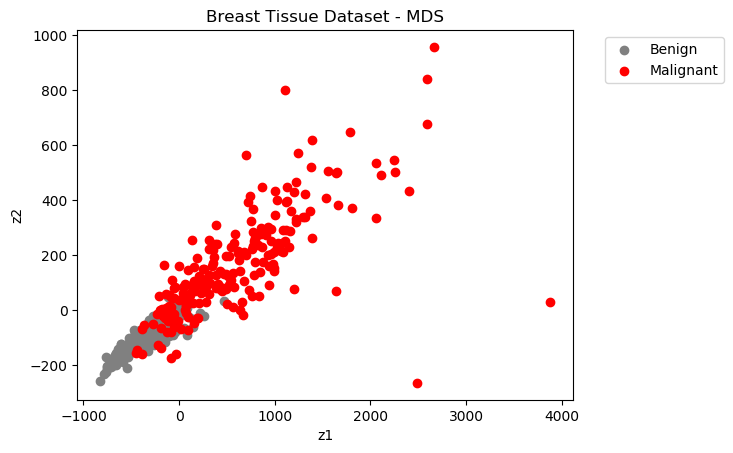
\includegraphics[width=0.49\textwidth]{../figs/mds_1}}
	\par\bigskip
	\subcaptionbox{ISOMAP, n\_neighbors = 5}{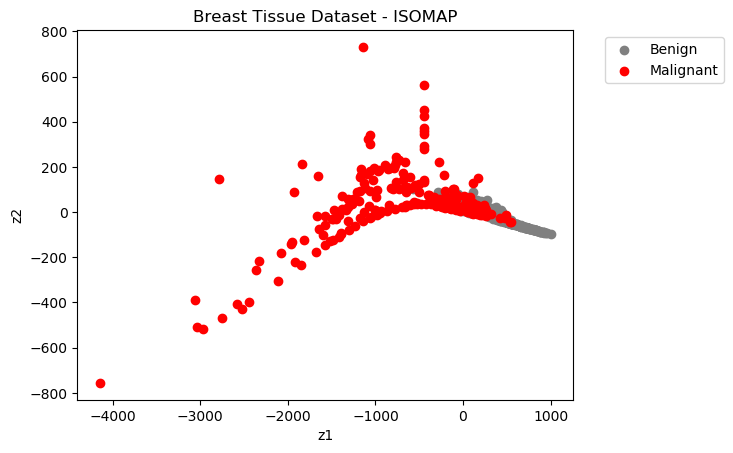
\includegraphics[width=0.49\textwidth]{../figs/isomap_1}}
	\subcaptionbox{T-distributed stochastic neighbour embedding}{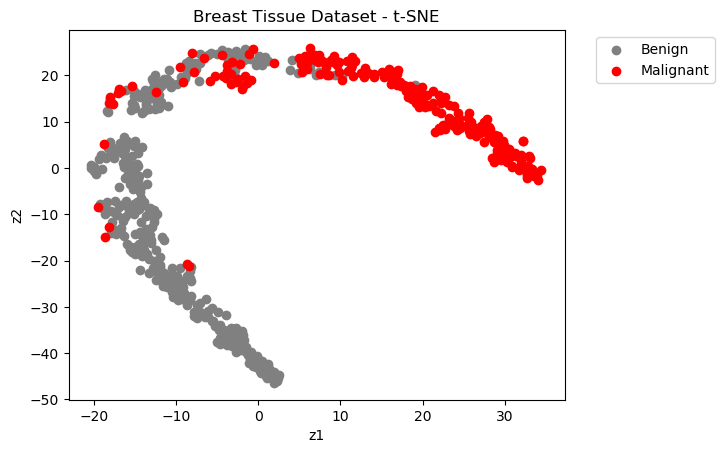
\includegraphics[width=0.49\textwidth]{../figs/tsne_1}}
	\caption{Visualizations obtained from unsupervised dimension reduction techniques}
	\label{fig:viz}
\end{figure}

\section{Discussion and Future Work}

Our supervised learning results show that each of the surveyed techniques perform well on the breast cancer dataset. We observe that each model achieves an average test error of less than 10\%. We also conclude that random forest classifiers perform the best on average for this dataset, with an average test error of approximately 4\%. 

Among our dimension reduction visualizations, t-distributed stochastic neighbour embedding arguably provides the most uniform clustering of the dataset. However, we still see significant regions of the visualization with a mix of malignant (cancerous) and benign (noncancerous) class labels. We therefore conclude that unsupervised dimension reduction is insufficient on its own to accurately classify breast tissue tumours, although it could lend support to a supervised classifier.

An important limitation of this project is the fact that only one dataset was examined and that it is limited to 569 examples. Future efforts could evaluate more datasets and perform more extensive hyperparameter tuning. While this project included a broad survey of machine learning techniques, it would be useful to deepen the investigation to include additional variations, such as kernel support vector machines. This would yield more definitive conclusions given the more extensive nature of the analysis.

Furthermore, increasingly complex tasks could be explored. It would be interesting to target datasets of tumour images directly with deep learning techniques such as convolutional neural networks. This would further streamline the diagnosis procedure and eliminate the need for a healthcare practitioner to manually compute the features from each image, as is the case with the dataset we used.

Despite these challenges, our work here affirms the usefulness of random forest classifiers for breast tissue classification amidst a wide array of machine learning algorithms. Medical software application developers are encouraged to consider random forests when applying machine learning  in their products.

%\section*{References}

\bibliographystyle{plainnat}
\bibliography{cancerDetection}

\end{document}
